\documentclass[border=10pt]{standalone}

\usepackage{tikz}
\usepackage{tikzsymbols}
\usetikzlibrary{calc,patterns,shapes.geometric}

\def\centerarc[#1](#2)(#3:#4:#5){\draw[#1] ($(#2)+({#5*cos(#3)},{#5*sin(#3)})$) arc (#3:#4:#5);}

\begin{document}
	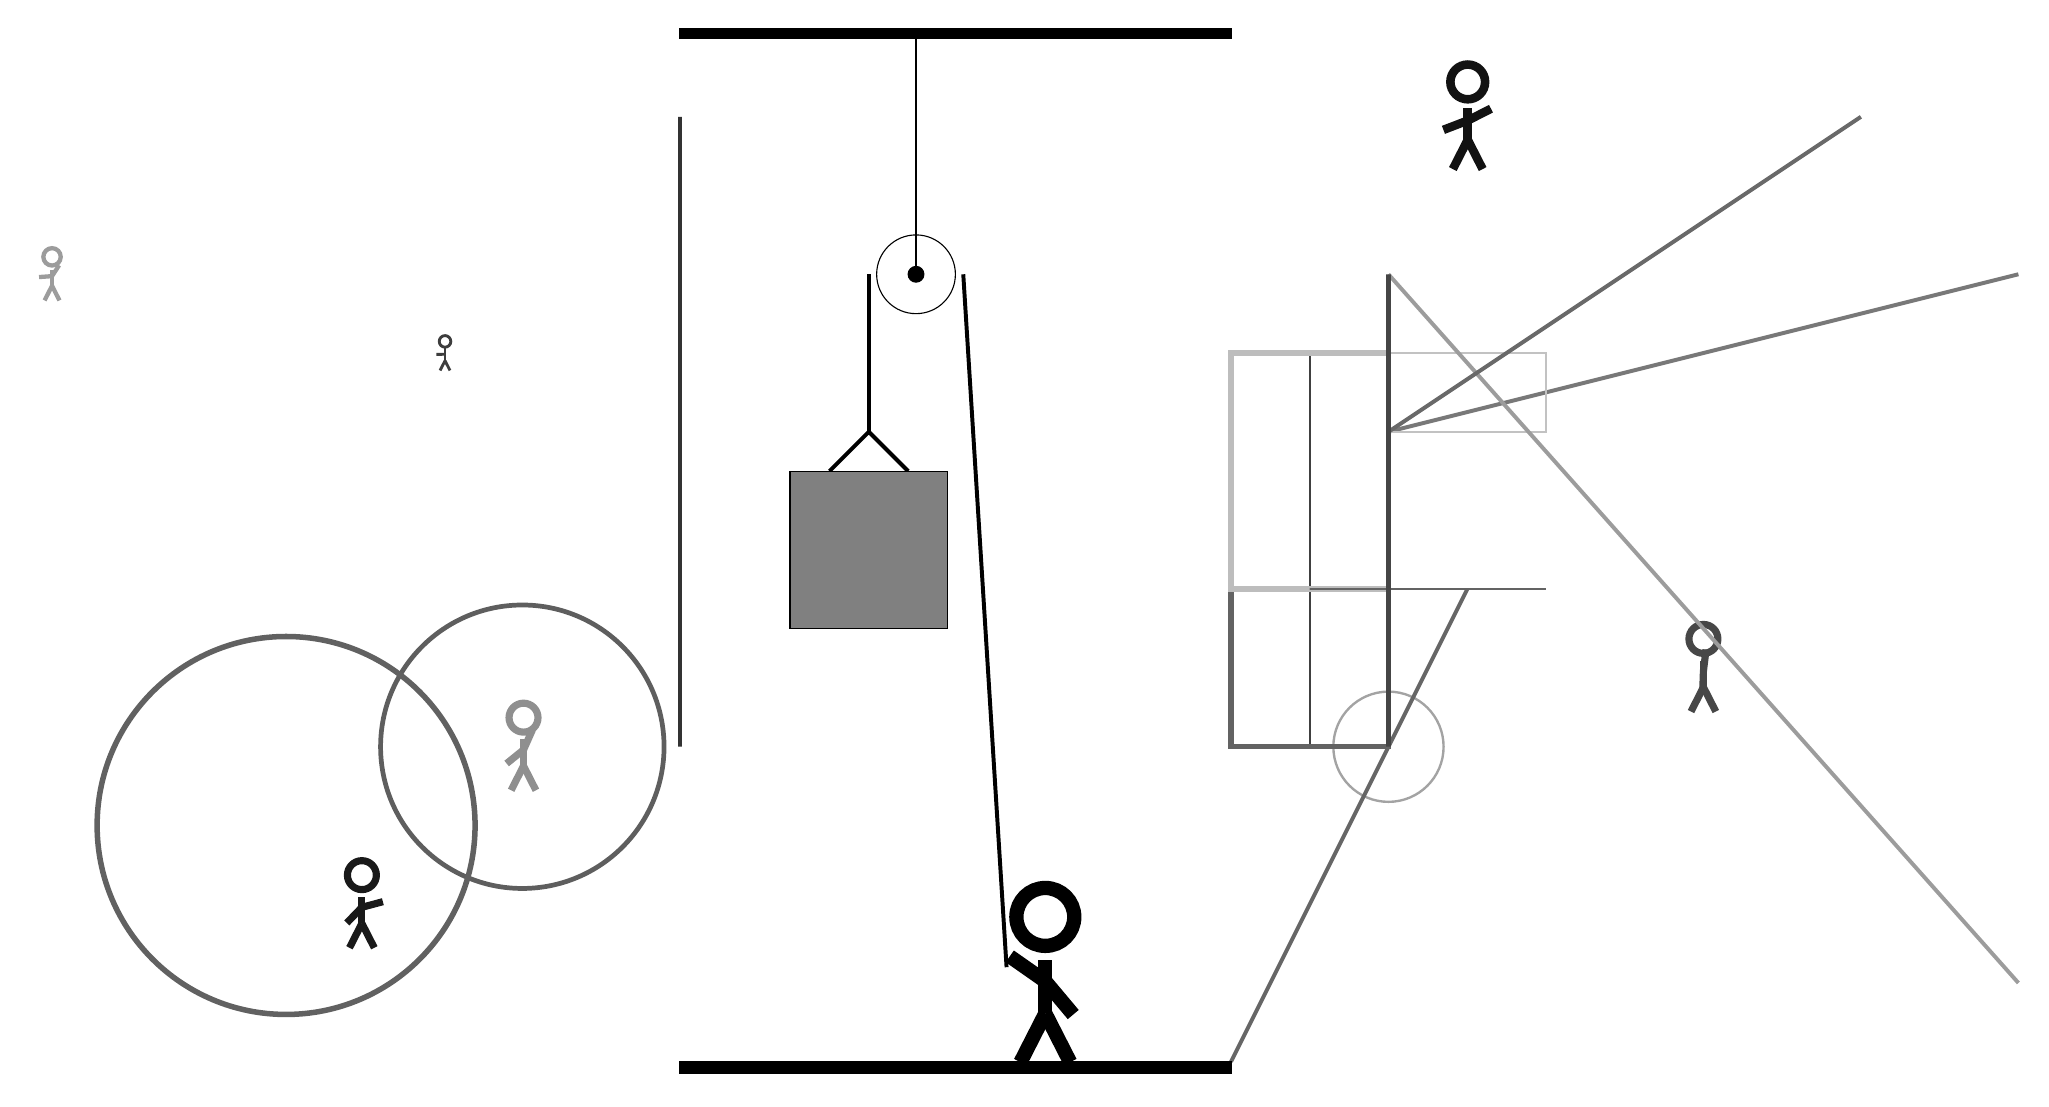
\begin{tikzpicture}
		%%%%% START %%%%%
		
		\draw[fill=black] (-2, 10) rectangle (5, 10.125);
		
		\draw[line width=0.5mm, color=black!53](7, 5) -- (15, 7);
		
		\node[line width=0.7mm, color=black!76] at (-5, 6) {\Strichmaxerl[2][1][90]};
		\node[line width=0.4mm, color=black!72] at (11, 2) {\Strichmaxerl[5][88][83]};
		\draw[line width=0.2mm, color=black!24] (7, 5) rectangle (9, 6);
		\draw [line width=0.6mm, color=black!63](-4, 1) circle (1.8);
		\draw[line width=0.3mm, color=black!75] (5, 6) rectangle (6, 1);
		\draw[line width=0.5mm, color=black!39](7, 7) -- (15, -2);
		\draw[line width=0.5mm, color=black!80] (-2, 9) rectangle (-2, 1);
		\draw [line width=0.3mm, color=black!36](7, 1) circle (0.7);
		\node[line width=0.4mm, color=black!39] at (-10, 7) {\Strichmaxerl[3][4][57]};
		\draw[line width=0.7mm, color=black!61] (5, 1) rectangle (7, 3);
		\draw[line width=0.7mm, color=black!26] (5, 3) rectangle (7, 6);
		\draw[line width=0.5mm, color=black!60](8, 3) -- (5, -3);
		
		\draw[line width=0.2mm, color=black!61] (6, 3) rectangle (9, 3);
		\node[line width=0.4mm, color=black!93] at (8, 9) {\Strichmaxerl[6][21][27]};
		\node[line width=0.3mm, color=black!90] at (-6, -1) {\Strichmaxerl[5][46][15]};
		
		\node[line width=0.7mm, color=black!44] at (-4, 1) {\Strichmaxerl[5][39][66]};
		\draw [line width=0.7mm, color=black!62](-7, 0) circle (2.4);
		\draw[line width=0.5mm, color=black!59](7, 5) -- (13, 9);
		
		\draw[line width=0.7mm, color=black!73] (7, 7) rectangle (7, 1);
		
		\draw (1, 7) circle (0.5);
		\draw[fill=black] (1, 7) circle (0.1);
		\draw (1, 10) -- (1, 7);
		
		\draw[line width=0.5mm] (-0.1, 4.5) -- (0.4, 5.0) -- (0.9, 4.5);
		\draw[fill=black!50] (-0.6, 4.5) rectangle (1.4, 2.5);
		
		\draw[line width=0.5mm] (0.4, 7) -- (0.4, 5.0);
		\centerarc[line width=0.5mm](1, 7)(0:180:0.6);
		\draw[line width=0.5mm](1.6, 7) -- (2.15, -1.8);
		
		\node at (2.6, -1.9) {\Strichmaxerl[10][-35][-50]};
		
		\draw[fill=black] (-2, -3) rectangle (5, -3.15);
		
		%%%%% END %%%%%
	\end{tikzpicture}
\end{document}